\subsection{The Star-Forming Sequence}
\label{sec:results:sfs}

Observations at both high- and low-$z$ suggest a tight relation between star formation rate and stellar mass, known as the `main sequence', or star-forming sequence \citep[SFS,][]{brinchmann_physical_2004,noeske_star_2007,speagle_highly_2014}.
The SFS is typically parametrised as a linear relation,
\begin{align}
  \mathrm{log_{10}(\SFR)} = \alpha \; \mathrm{log_{10}(M_{*}\,/\, M_{\odot})} + \beta\;\;.
\end{align}
Observations suggest that the normalisation $\beta$ increases with redshift, whilst the slope $\alpha$ remains relatively constant \citep{daddi_multiwavelength_2007, santini_star_2009, salmon_relation_2015}.


There have been suggestions of a turnover in the SFS at high stellar masses, though the turnover mass, and its evolution with redshift, are less clear \protect\citep{lee_turnover_2015,tasca_evolving_2015,santini_star_2017}.
Such a turnover is necessary to explain the GSMF at low redshift; a single power law slope would lead to too many massive galaxies being formed \citep[between $10^{10} < \mathrm{M_{*}/M_{\odot} < 10^{11}}$,][]{leja_reconciling_2015}.
% A turnover has also been conspicuosly absent from models \citep[\textit{e.g.} Illustris, ][]{sparre_star_2015}.
The turnover may be evidence for a change in the dominant channel of stellar mass growth, from smooth gas accretion to merger-driven growth.

\begin{figure}
	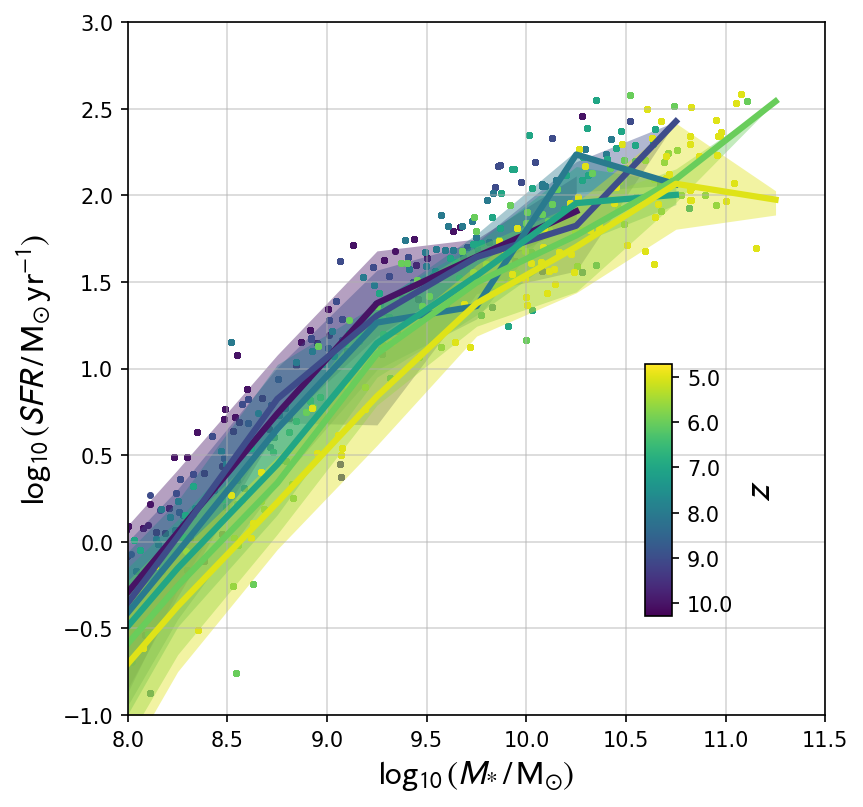
\includegraphics[width=\columnwidth]{images/sfs_all.png}
  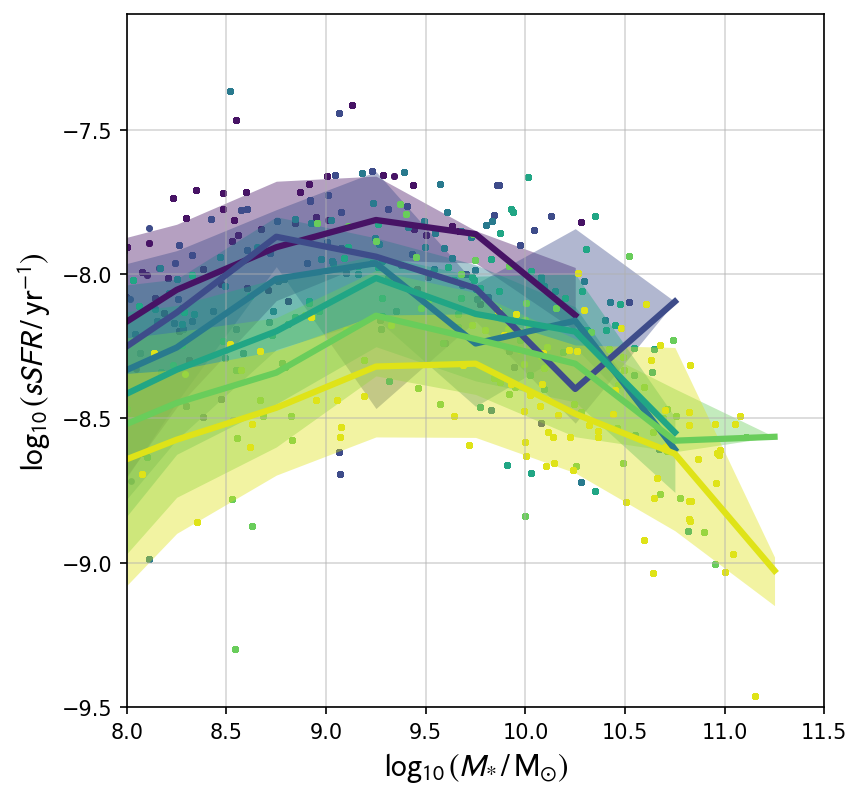
\includegraphics[width=\columnwidth]{images/ssfr_all.png}
    \caption{\textit{Top:} Redshift evolution of the \flares\ composite star forming sequence.
    Solid lines show the weighted composite SFS for centrals + satellites, with the 16$^{\mathrm{th}}$-84$^{\mathrm{th}}$ spread shaded.
    Points show individual central galaxies.
    \textit{Bottom:} as for the top panel, but showing the specific-star formation rate - stellar mass relation.
    }
    \label{fig:sfs_all}
\end{figure}

The top panel of \fig{sfs_all} shows the redshift evolution of the SFS in \flares.
In the bottom panel of \fig{sfs_all} we also show the specific-star formation rate (sSFR) against $M_{*}$ relation.
To construct the median lines, we weight each galaxy in the sample by the appropriate factor for the overdensity of the resimulation volume, as described in \Sec{method:weighting}.\footnote{In fact, as shown in \Fig{sfs_overdensity}, the environmental dependence is very weak and so the weighted relations are very similar to the unweighted ones.}
There is a clear trend of decreasing normalisation with decreasing redshift, approximately $0.5$ dex between $z = 10 \,-\, 5$.
There is some noise in the weighted relation at $z = 8$ for galaxies with $M_{*} > 10^{9.5} \, M_{\odot}$; we checked, and found that this is due to a small number of galaxies in mean density regions above this mass limit with low SFRs, biasing the normalisation down.

We have not excluded `passive' galaxies from our measurement of the SFS.
We present results for the SFS assuming different specific-SFR cuts in \app{ssfr_cut}, though note here that they make negligible difference to the relations at $z \geqslant 5$ for even the most liberal cuts.


\begin{figure}
	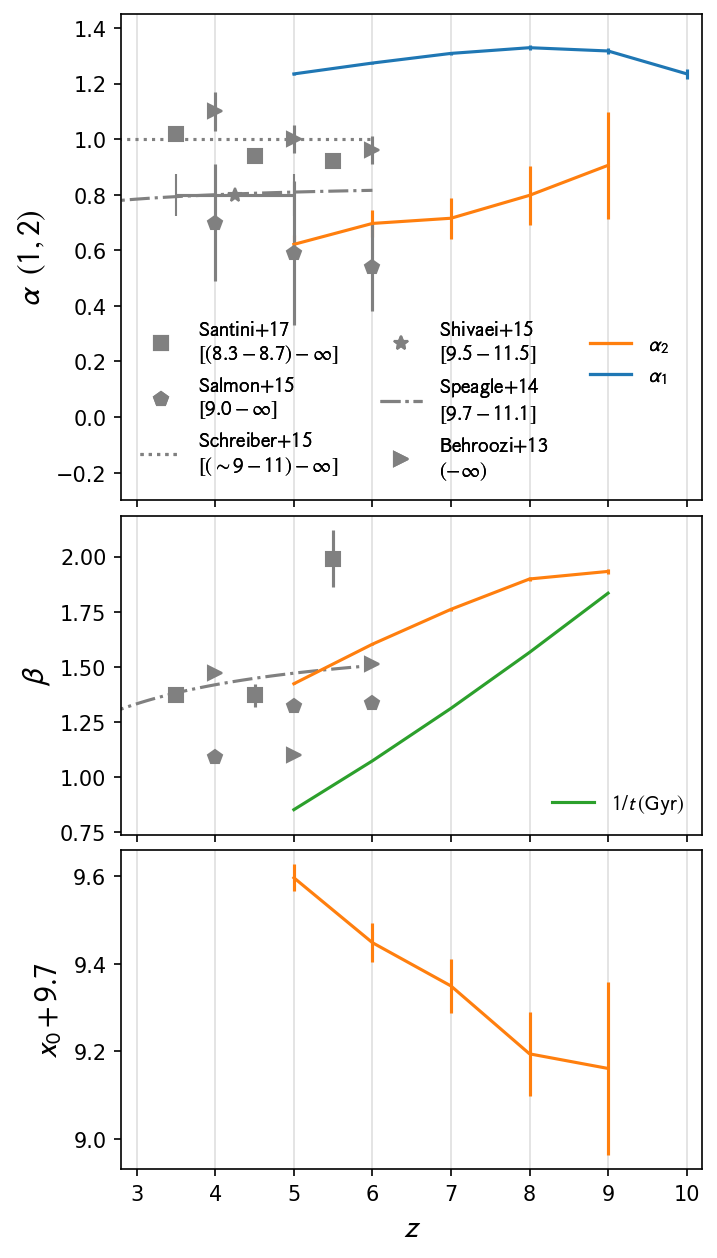
\includegraphics[width=\columnwidth]{images/sfs_fit_evolution.png}
    \caption{Redshift evolution of the piecewise-linear fit to the SFS.
    Observational results are plotted where available in grey, from \protect\cite{behroozi_average_2013,speagle_highly_2014,shivaei_mosdef_2015,salmon_relation_2015,schreiber_herschel_2015,santini_star_2017}.
    The lower- and upper-mass completeness limits for these studies are quoted in the legend.
    \textit{Top}: high- and low-mass slope, in orange and blue respectively.
    \textit{Middle}: normalisation, $\beta$, in orange.
    The inverse age of the universe in Gyr is shown in green; the normalisation approximately follows the same relation, but with a slightly shallower evolution.
    \textit{Bottom}: turnover mass in log-solar masses, in orange.
    }
    \label{fig:sfs_fit_evolution}
\end{figure}


There is a clear turnover in the \flares\ star-forming sequence at high masses ($\sim \,>\, 10^{9.3} \mathrm{M_{\odot}}$).
We account for this by fitting a piecewise-linear relation, with an upper- and lower-mass part, for stellar mass re-normalised at $10^{9.7} \mathrm{M_{\odot}}$,
\begin{align}
	\log_{10}\SFR = \alpha_{1} \, \mathrm{log_{10}}(M_{*}\,/\,10^{9.7} \mathrm{M_{\odot}}) + \beta_{1} \quad & x \leqslant x_{0} \\
	\log_{10}\SFR = \alpha_{2} \, \mathrm{log_{10}}(M_{*}\,/\,10^{9.7} \mathrm{M_{\odot}}) + \beta_{2} \quad & x \geq x_{0} \;,
\end{align}
where $\alpha_{1}$ is the low-mass slope, $\alpha_{2}$ is the high-mass slope, and $x_{0}$ is the turnover mass in log-solar masses. The normalisation at the turnover, $\beta_{0}$, is then given by
\begin{align}
\beta_{0} & = \beta_{2} + \alpha_{2} \, x_{0} \\
& = \beta_{1} + \alpha_{1} \, x_{0} \;\;.
\end{align}

We use the \textsc{scipy} implementation of non-linear least squares to perform the fit, combined with a non-parametric bootstrap approach for estimating parameter uncertainties.
The bootstrap is implemented as follows: we select, with replacement, 500 times from the original data, each resample being the same size as the original data.
We then fit each sample independently; parameter estimates are given by the median of the resampled fit distributions, and uncertainties are given as the 1$\sigma$ spread in the distributions (unless otherwise stated).
The parameter fits are quoted in \protect\tab{sfs_params}.

\begin{figure}
	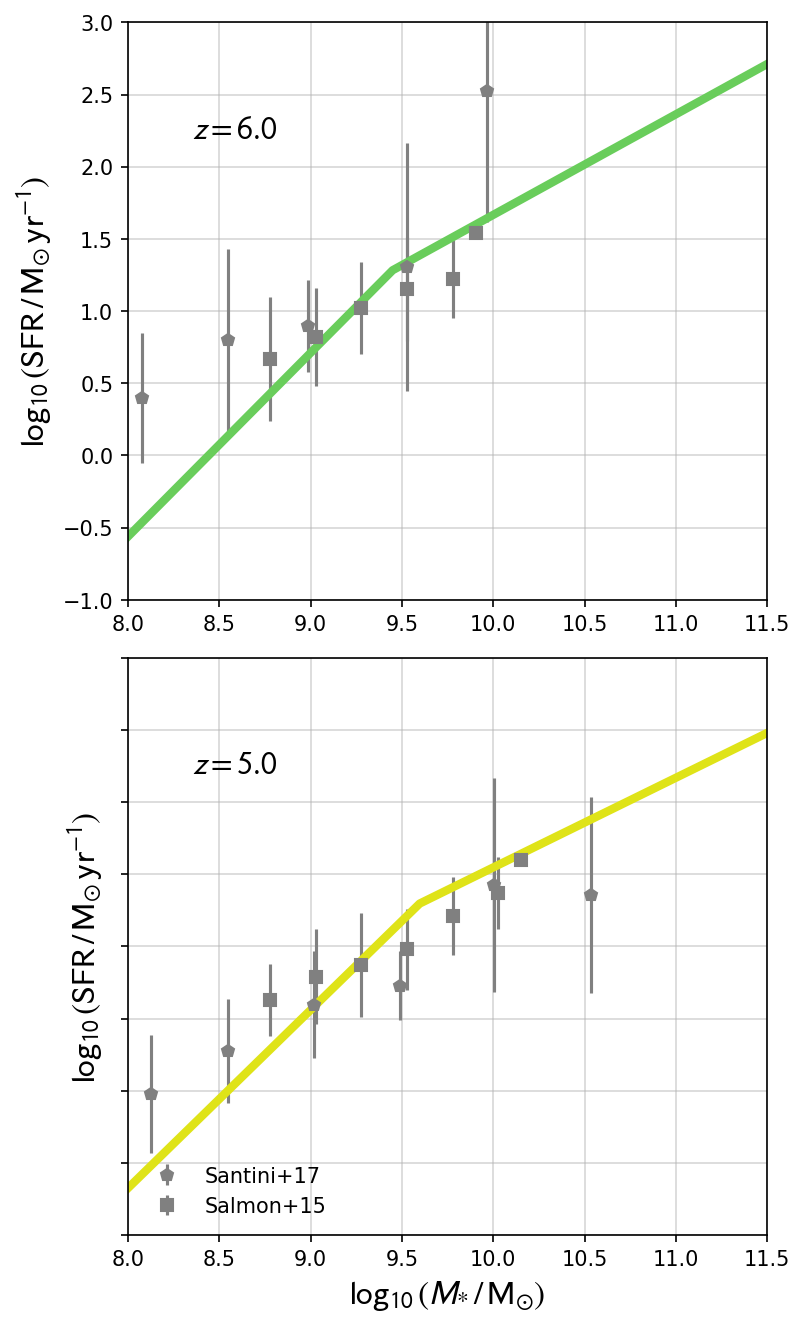
\includegraphics[width=\columnwidth]{images/sfs_obs.png}
    \caption{\flares\ composite SFS at $z = 5.0$ and $6.0$ compared to high redshift observational constraints from \protect\cite{santini_star_2017} and \protect\cite{song_evolution_2016}.
    }
    \label{fig:sfs_obs}
\end{figure}

\protect\fig{sfs_fit_evolution} shows the redshift evolution of each parameter against observational constraints where available.\footnote{The high mass slope and turnover are poorly constrained at $z = 10$ so we omit them.}
There are few robust observational constraints at $z > 6$, so we show constraints down to $z = 3$ to provide context to the redshift evolution \citep{behroozi_average_2013,schreiber_herschel_2015,shivaei_mosdef_2015,salmon_relation_2015,santini_star_2017}, including the compilation of pre-2014 measurements from \cite{speagle_highly_2014}.
These all represent single power-law measurements.
For all observations we quote the approximate lower mass completeness limit for the whole fit in the legend.
We also show a direct comparison of the fits to binned data from \cite{santini_star_2017} and \cite{salmon_relation_2015} in \fig{sfs_obs} at $z = 5\,-\,6$.

The normalisation is within the errors of the binned observations at these redshifts.
The fitted normalisation $\beta$ is also within the spread of the fitted relations at these redshifts, and continues the apparent increasing normalisation with increasing redshift from $z = 3$.
We also show the inverse age of the Universe (in Gyr); the fall in SFS normalisation approximately follows the same relation, but slightly shallower.

The slope of the observed relations shows considerable scatter spanning the range $\sim \, 0.5 - 1.1$.
We suggest that this is due to the lower-mass limit of these observations (quoted in the legend of \fig{sfs_fit_evolution}).
Since these studies fit a single power-law, and assume a high lower-mass completeness limit, ($M_{*} \,/\, M_{\odot} > 10^{9.5}$), the measured slope will be biased to shallower slopes.
This can also be seen clearly in the binned relations in \fig{sfs_obs}; both \cite{santini_star_2017} and \cite{song_evolution_2016} straddle the turnover mass in \flares.
Finally, this can also be seen in the redshift evolution of these studies.
The observed slopes of \cite{salmon_relation_2015}, \cite{behroozi_average_2013} and \cite{santini_star_2017} all show a negative correlation with redshift.
The lower-mass completeness limit of these studies also increases with increasing redshift; as it increases, they tend to probe just the high-mass end of the SFS, rather than the steeper low-mass end.
This suggests that many high redshift measures of the SFS, where the mass completeness does not extend to very low masses, are only probing the SFS at stellar masses above the turnover, and the measured slopes do not represent a universal relation for all masses.

The turnover mass shows a negative correlation with redshift, increasing from $\sim 10^{9.2}$ to $10^{9.6} \, M_{*} \,/\, M_{\odot}$ between $z = 9 - 5$.
There are unfortunately no observational constraints on the turnover mass at $z > 3$.
We note that the turnover mass is much lower than that measured in low-$z$ studies  \citep[$> 10^{10} \, M_{*} \,/\, M_{\odot}$ at $z \leqslant 3$,][]{whitaker_constraining_2014,tasca_evolving_2015}.


\subsubsection{Environmental dependence of the SFS}

\begin{figure}
	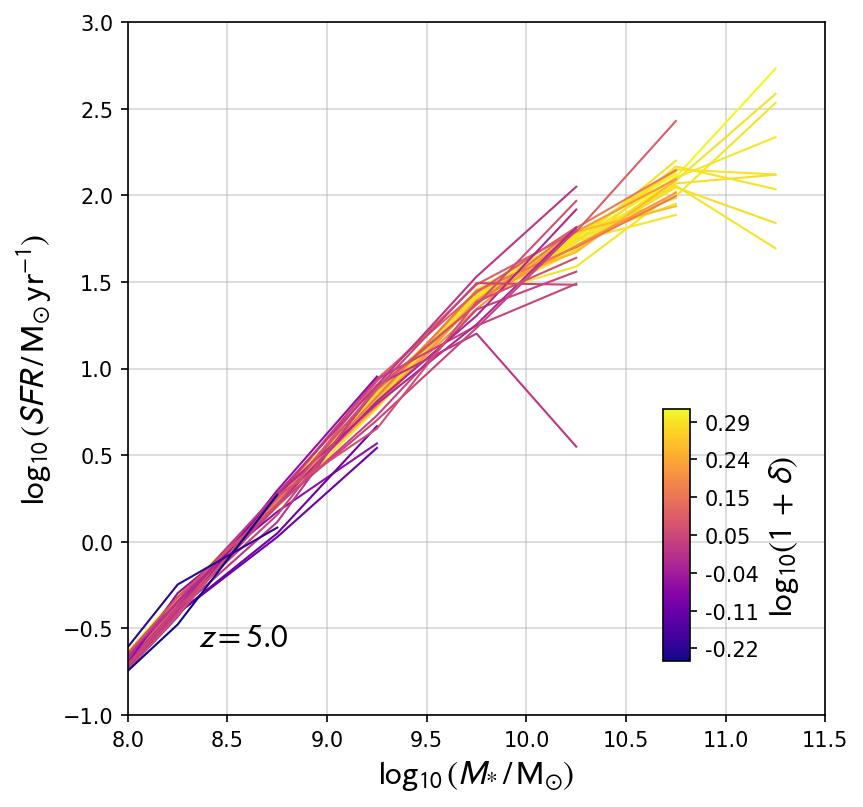
\includegraphics[width=\columnwidth]{images/sfs_overdensity.png}
    \caption{SFS for each region at $z = 5$, coloured by overdensity.
    }
    \label{fig:sfs_overdensity}
\end{figure}

\fig{sfs_overdensity} shows the SFS for each region individually at $z = 5$, coloured by overdensity.
The highest overdensities reach to higher stellar masses, as expected.
However, there is no dependence on overdensity of either the normalisation nor shape of the SFS, and we see this up to $z = 10$.
This matches observational comparisons between high density and field regions at $z \sim 2$
\citep{koyama_evolution_2013,koyama_environmental_2014,shimakawa_mahalo_2017,shimakawa_mahalo_2018}, though these authors do note some differences in dense subgroups in protocluster candidates.
We leave a study of the small-scale overdensity dependence of the SFS to future work.
